% 2  Previous Work
% 2.1  Problem setup picture(s) (which shows all variables)
% 2.2  Assumptions
% 2.3  NLSWEs ? derived from conservation of mass and Newton?s Second Law under assumptions (Just mention, not actually derive)
% 2.3.1  Mention that the SWEs have no dispersion ? there is very little dispersion near shore so this is where SWEs apply? fact check and/or more info
% 2.4  Very brief overview of how NLSWEs are linearized for arbitrary cross section
% 2.4.1  Properties of new system
% 2.4.2  Include equations to get back to physical variables
% 2.4.3  Analytical F(?) and thus W(?) for |y|^m case


\section{Previous Work}
	\begin{frame}
		\frametitle{Introduction to the Bay Shapes}
		In the field of Tsunami run-up research, there are several natural bay shapes to examine:
		\begin{itemize}
			\item The plane beach;
			\item Bays of parabolic cross-section;
			\item Bays of trapezoidal cross-section.
		\end{itemize}
		There has been extensive study of the plane beach and bays of parabolic cross-section, but tsunami behavior in bays of trapezoidal cross-section has not yet been examined.
		
		In each case, we assume that the bottom profile is separable: \emph{i.e.}
		\[   z(x,y) = f(y) - h(x)  \]
		where $z(x,y)$ is the bottom profile, $f(y)$ is an arbitrary function and $h(x)$ is an arbitrary non-negative function.
	\end{frame}

	\slide[The Plane Beach]{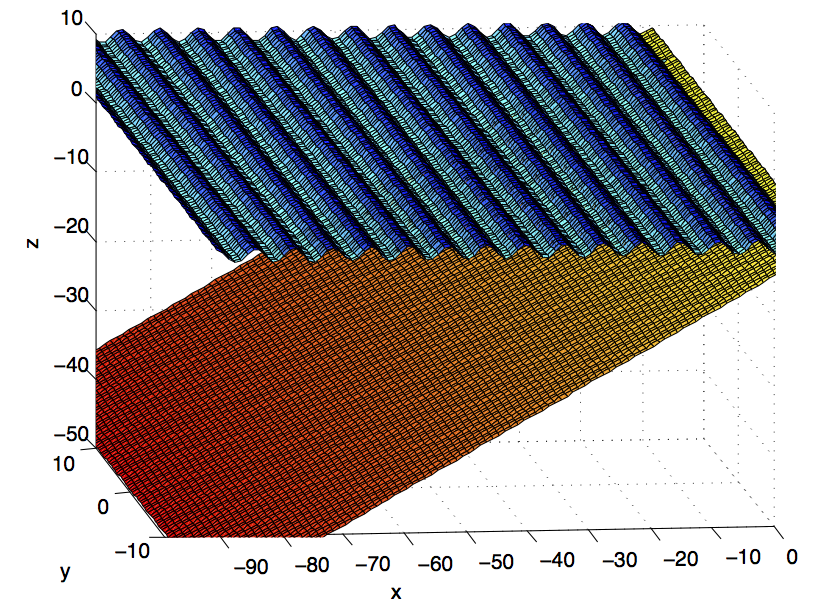
\includegraphics[width=\linewidth]{bay/planebeach.png}}

	\begin{frame}
	\frametitle{The Plane Beach}
		Characteristics of the plane beach:
		\begin{itemize}
			\item Potentially non-constant slope;
			\item Uniform across y-axis;
			\item Can be simplified to 2 dimensions.
		\end{itemize}
		This is the problem examined in the famous 1958 paper of Carrier and Greenspan. They showed that in this case, explicit solutions to the shallow water wave equations were possible.
	\end{frame}

	\slide[Bays of Parabolic Cross-section]{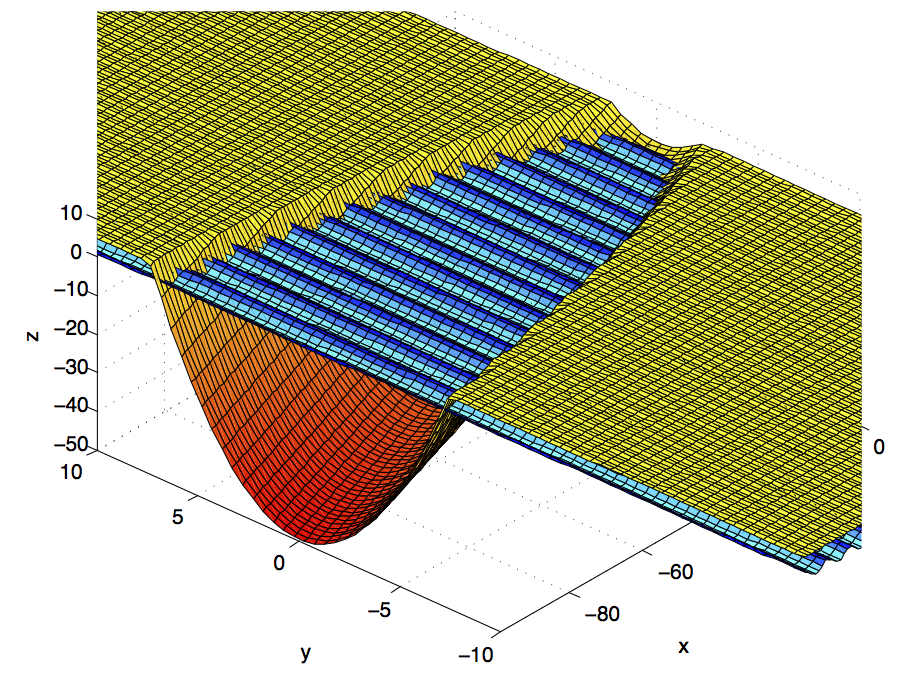
\includegraphics[width=\linewidth]{bay/parabolicbay.png}}

	\begin{frame}
		\frametitle{Bays of Parabolic Cross-section}
		Characteristics of bays of parabolic cross-section:
		Characteristics of bays of parabolic cross-section:
		\begin{itemize}
			\item Constant slope;
			\item Parabolic cross-section along y-axis;
			\item Behavior of waves in such a channel can still be simplified to 2 dimensions.
		\end{itemize}
		This more complicated problem was analyzed in a recent paper by Dr. Ira Didenkulova and Dr. Efim Pelinovsky, in which they showed that it was possible to reduce this problem to one that is analogous to the 2-dimensional case, and thus analytical solutions are possible.
	\end{frame}

	\slide[Bays of Trapezoidal Cross-section]{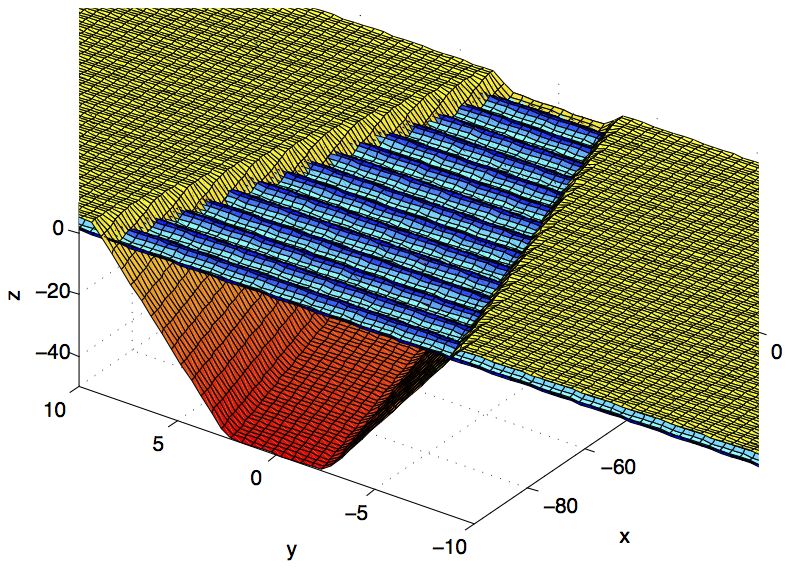
\includegraphics[width=\linewidth]{bay/trapezoidalbay.png}}

	\begin{frame}
		\frametitle{Bays of Trapezoidal Cross-section}
		%Insert a graphic of a trapezoidal cross-section'd bay here. Float left.
		Characteristics of bays of trapezoidal cross-section:
		\begin{itemize}
			\item Constant slope
			\item Cross-section is determined by a symmetrical trapezoid\\
			slope of the walls is $\beta$\\
			distance across the base is $2 y_0$
			\item Behavior of waves in such a bay is unknown. 
		\end{itemize}
		These bays where the focus of the previous REU.
	\end{frame}

	\begin{frame}
		\frametitle{Terminology}
		\begin{itemize}
			\item $\eta(x,t)$ is the perturbation of water level at time $t$, distance $x$ from shore.
			\item $H(x,t)$ is the total water depth. Note: $H(x,t) = h(x) + \eta(x,t)$.
			\item $S(H)$ is the cross-sectional area of the bay. Note
				\[ S(H) = \int_0^{H(x,t)} f(y) \delta y \]
			\item $u(x,t)$ is the average water velocity on a cross-section perpendicular to the cross-section.
			\item We only consider $h(x) = -\alpha x$, where $\alpha$ is a non-negative constant. Since $x$ is typically negative in our domain, $h$ will usually be non-negative, and $H$ must always be non-negative.
		\end{itemize}
	\end{frame}
	\begin{frame}
		\frametitle{Shallow-Water Wave Equations}
		Assuming that there is no lateral fluid motion:
		\begin{framed} \begin{align}
			\label{swe1} S_t + (uS)_x &= 0\\
			\label{swe2} u_t + u u_x + g H_x &= g h_x
		\end{align} \end{framed}
		%swe1 is conservation of mass
		%swe2 is conservation of momentum
		We have initial conditions that at $t=0$, $u(x,0) = 0$ and $\eta(x,0) = \eta_0(x)$, and boundary conditions that as $x$ becomes large, $u$ and $\eta$ become small, and that at the moving shoreline, $u(x,t)$ is bounded.
	\end{frame}

	\slide[Conversion to Matrices] {
		Noting that because $S(H) = \int_0^{H(x,t)} f(y) \delta y$, $S_t = S_H H_t$ and $S_x = S_H H_x$.
		\begin{align*}
			A_H H_t + A_H u H_x + A u_x &= 0\\
			u_t + g H_x + u u_x &= g h_x
		\end{align*}
		dividing the top equation by $A_H$, we have the following system
		\[
			\left [ \begin{array}{ccc} H \\ u \end{array} \right ]_t
			+ \left [ \begin{array}{ccc} u & A/A_H \\ g & u \end{array} \right ]
				\left [ \begin{array}{ccc} H \\ u \end{array} \right ]_x
			= \left [ \begin{array}{ccc} 0 \\ gh_x \end{array} \right ]
		\]
		which will be referred to as
		\begin{align}
			\label{sweMat1} v_t + X v_x = b
		\end{align}
	}
	\slide[Characteristic Equation] {
		Assuming there's a characteristic function $c(x,t)$
		\[v_s = v_x x_s + v_t t_s \]
		substituting in \eqref{sweMat1}
		\begin{align*}
			 v_s &= v_x x_x + (b - X v_x) t_s \\
			&= (I x_s - X t_s) v_x + b t_s
		\end{align*}
	}
	\slide[Eigenvectors] {
		If $(I x_s - X t_s)$ is nonsingular, then our solutions are trivial (zero). Thus, for non-trivial solutions
		\[ | I x_s - X t_s | = 0 \]
		then we can solve for $x_s$
		\[ x_s = (u \pm \sqrt{g A / A_H}) t_s = \lambda_\pm t_s \]
		if we set $t_s = 1$
		\[ v_s = (I \lambda_\pm - X) v_x + b \]
		Eigenvector decomposition
		\[ V_\pm^\ast X = \lambda_\pm V_\pm^\ast ,
			\qquad \text{where} V_\pm^\ast = \mat{ \pm \sqrt{g A_H / A} \\ 1} \]
	}
	\slide[Riemann Invariants] {
		The Riemann Inveriants are derived from the eigenvectors
		\[ V_\pm = \mat{ \pm \sqrt{g A_H / A} \\ 1} = \mat{I_H \\ I_u},
			\qquad I_\pm = u \pm \int \sqrt{g A_H / A} \cdot dH \]
		note that
		\[ V_\pm^\ast v_z = \mat {I_H & I_u} \mat{H \\ u}_z = I_z \]
		thus
		\begin{align*}
			V^\ast_\pm(v_t + X v_x) &= V_\pm^\ast b \\
			I_t + \lambda_\pm I_x &= g h_x \\
			(\pderiv{}{t} + \lambda_\pm \pderiv{}{x})(I_\pm - g h_x t)
		\end{align*}
		we're using constant sloped bays, so $h=\alpha x$ and $h_x = \alpha$.
	}
	\slide[Hodograph Transform] {
		
	}

\begin{frame}
\frametitle{Hodograph Transform}
We apply a hodograph transform with Jacobian $\dfrac{\partial (t,x)}{\partial(I_+, I_-)}$. This Jacobian will be zero if, and only if, the wave breaks before it reaches shore. After applying the transform, we see that
\[
\frac{\partial(I_\pm,x)}{\partial(I_+,I_-)} + c_\pm \frac{\partial (t, I_\pm)}{\partial(I_+,I_-)} = 0,
\]
which can be written as
\begin{equation}\label{hodograph}
\frac{\partial x}{\partial I_\pm} - c_\mp \frac{\partial t}{\partial I_\pm} = 0.
\end{equation}
\end{frame}

\begin{frame}
\frametitle{Change of Variables}
We define two new variables:
\[
\lambda = \frac{I_+ + I_-}{2} \text{ and } \sigma = \frac{I_+ - I_-}{2}.
\]
Notice that this implies that
\begin{equation} \label{siglam}
\lambda = u + \alpha g t \text{ and } \sigma = \int_0^H \sqrt{\frac{g}{S} \frac{dS}{dH}}dH.
\end{equation}
We also define
\[
F(\sigma) = c_+ - c_- = 2 \sqrt{gS \frac{dH}{dS}}.
\]
\end{frame}

\begin{frame}
\frametitle{Change of Variables}
In these new variables, \eqref{hodograph} becomes
\[
\frac{\partial^2 t}{\partial \lambda^2} - \frac{\partial^2 t}{\partial \sigma^2} - \left( \frac{2 + \frac{dF}{d\sigma}}{F(\sigma)} \right) \frac{\partial t}{\partial \sigma} = 0,
\]
which, because of how $u,t,$ and $\lambda$ are related in \eqref{siglam}, is equivalent to
\begin{equation}\label{finalu}
\frac{\partial^2 u}{\partial \lambda^2} - \frac{\partial^2 u}{\partial \sigma^2} - \left( \frac{2 + \frac{dF}{d\sigma}}{F(\sigma)} \right) \frac{\partial u}{\partial \sigma} = 0.
\end{equation}
So we can find $t$ and $u$.
\end{frame}

\begin{frame}
\frametitle{Finding a relation for $x$}
In order to find $x$, we also obtain from \eqref{hodograph} that
\[
g \alpha \frac{\partial x}{\partial \sigma} = - u \frac{\partial u}{\partial \sigma} - \frac{F(\sigma)}{2} + \frac{F(\sigma)}{2} \frac{\partial u}{\partial \lambda}.
\]
To integrate this, we define $\Phi(\sigma,\lambda)$ by
\[
u = \frac{1}{F(\sigma)} \frac{\partial \Phi}{\partial \sigma}.
\]
Then we see that
\[
2 g \alpha x = \frac{\partial \Phi}{\partial \lambda} - \int_0^\sigma F(\sigma) d\sigma - u^2 = \frac{\partial \Phi}{\partial \lambda} - 2gH - u^2.
\]
Hence
\[
\eta = H - h = H + \alpha x = \frac{1}{2g} \left(\frac{\partial \Phi}{\partial \lambda} - u^2 \right)
\]
\end{frame}

\begin{frame}
\frametitle{Finding $\Phi$}
We substitute our definition of $\Phi$ into \eqref{finalu} to obtain
\begin{equation}\label{Phieq}
\frac{\partial^2 \Phi}{\partial \lambda^2} - \frac{\partial^2 \Phi}{\partial \sigma^2} - W(\sigma) \frac{\partial \Phi}{\partial \sigma} = 0,
\end{equation}
where
\[
W(\sigma) = \frac{2 + \frac{dF}{d\sigma}}{F(\sigma)}.
\]
We can think of $\sigma$ as a space-like variable and $\lambda$ as a time-like variable. So we have initial conditions at $\lambda = 0$,
\[
\frac{\partial \Phi(\sigma,0)}{\partial \sigma} = 0 \text{ and } \frac{\partial \Phi(\sigma,0)}{\partial \lambda} = 2g\eta_0.
\]
Our boundary conditions are
\[
\frac{\partial \Phi(\infty,\lambda)}{\partial \sigma} = 0 \text{ and } \frac{\partial \Phi(0,\lambda)}{\partial \sigma} = 0.
\]
\end{frame}

\begin{frame}
\frametitle{Introducing $\varphi$ and $\psi$}
We define two new variables:
\[
\varphi = \frac{\partial \Phi}{\partial \lambda} \text{ and } \psi = \frac{\partial \Phi}{\partial \sigma}.
\]
Notice that by the equality of second partial derivatives, $\dfrac{\partial \varphi}{\partial \sigma} = \dfrac{\partial \psi}{\partial \lambda}$.
By substituting $\varphi$ and $\psi$ into \eqref{Phieq}, we obtain
\[
\frac{\partial \varphi}{\partial \lambda} - \frac{\partial \psi}{\partial \sigma} - W(\sigma) \psi = 0.
\]
Finally, we define $\Omega = \begin{pmatrix} \varphi \\ \psi \end{pmatrix}$.
\end{frame}

\begin{frame}
\frametitle{The system in $\Omega$}
We have the system of equations
\[
\dfrac{\partial \psi}{\partial \lambda} = \dfrac{\partial \varphi}{\partial \sigma} \text{ and } \frac{\partial \varphi}{\partial \lambda} = \frac{\partial \psi}{\partial \sigma} + W(\sigma) \psi.
\]
In matrix form, this is
\[
\Omega_\lambda = \begin{pmatrix} 0 & 1 \\ 1 & 0 \end{pmatrix} \Omega_\sigma + \begin{pmatrix} 0 & W \\ 0 & 0 \end{pmatrix} \Omega.
\]
We also have initial conditions
\[
\psi(\sigma, 0) = 0 \text{ and } \varphi(\sigma,0) = 2g\eta_0
\]
and boundary conditions
\[
\psi(\infty,\lambda) = 0 \text{ and } \psi(0,\lambda) = 0.
\]
\end{frame}

\begin{frame}
\frametitle{Backsubstituting to Physical Variables}
We have the following backsubstitution equations:
\[
u = \frac{\psi}{F(\sigma)} \text{ and } \eta = \frac{1}{2g}\left(\varphi - u^2\right)
\]
\[
x = \frac{1}{2g\alpha} \left(\varphi - 2gH - u^2 \right) \text{ and } t = \frac{\lambda - u}{\alpha g}.
\]
We know that this backsubstitution is possible because the 4-part Jacobian matrix
\[
\frac{\partial (x,t,u,\eta)}{\partial (\sigma,\lambda,\psi,\varphi)}
\]
has a non-zero determinant.
\end{frame}

\section{Analytics}

\begin{frame}
\frametitle{Known Analytics}
From \eqref{Phieq}, the shallow water equations for the parabolic bay are: 
\[
\frac{\partial^2 \Phi}{\partial \lambda^2}-\frac{\partial^2 \Phi}{\partial \sigma^2}-\frac{2}{\sigma}\frac{\partial \Phi}{\partial \sigma}=0.
\]
Where we can find $u$, $\eta$ , $x$ and $t$ by the following non-linear transforms:\\
\begin{align*}
u=\frac{1}{\sigma}\frac{\partial \Phi}{\partial \sigma}&, \eta=-\frac{1}{g}\left(\frac{u^2}{2}-\frac{1}{3}\frac{\partial \Phi}{\partial \lambda}\right)\\
t=\frac{u-\lambda}{g\alpha}&,x=\frac{1}{g\alpha}\left(\frac{u^2}{2}+\frac{\sigma^2}{6}-\frac{1}{3}\frac{\partial \Phi}{\partial \lambda}\right)
\end{align*}
\end{frame}


\begin{frame}
\frametitle{Known Analytics Cont.}
We solve this in the semi-axis $\sigma \geq 0$ with the following conditions: \\
\begin{align*}
IC's:& \Phi|_{\lambda=0}=0\\
&\frac{\partial\phi}{\partial \lambda}|_{\lambda=0}=\frac{\sigma^2}{2}-3g\alpha x(\sigma)|_{\lambda=0}\\
\end{align*}
Where $\Phi|_{\lambda=0}=0$ because the initial averaged cross-sectional water velocity is 0. We know the initial water height as $\sigma=\sqrt{6gH}$.
\\ \vspace{3mm}
BC's: Boundedness of water displacement and velocity at the shoreline and at infinity.
\end{frame}

\begin{frame}
\frametitle{Known Analytics Cont.}
The solution to this is:\\\vspace{7mm}
$\Phi(\sigma,\lambda)=\frac{[\Theta(\lambda+\sigma)-\Theta(\lambda-\sigma)]H(\lambda-\sigma)-[\Theta(\sigma+\lambda)-\Theta(\sigma-\lambda)]H(\sigma-\lambda)}{\sigma}$\\\vspace{3mm}
Where $H$ is the Heaviside function and $\Theta$ is determined by the initial wave function.
\end{frame}

\begin{frame}
\frametitle{An Example run up problem}
Let $\Theta(\sigma)=A e^{-(\frac{\sigma-\sigma_0}{p})^2}$ where $A$ is the wave height, $p$ is the wave length, and $\sigma_0$ represents the distance of the wave from the shore.\\
The solution for this initial wave is:\\
\begin{align*}
\Phi(\sigma\geq0,\lambda)=&\frac{A}{\sigma} \left[ e^{-(\frac{\sigma+\lambda-\sigma_0}{p})^2}-e^{-(\frac{\sigma-\lambda-\sigma_0}{p})^2} \right. \\
&\left. +e^{-(\frac{\sigma+\lambda+\sigma_0}{p})^2}-e^{-(\frac{\sigma-\lambda+\sigma_0}{p})^2} \right]
\end{align*}
\end{frame}

\begin{frame}
\frametitle{Maximum/Minimum run up/run down}

For our N-Wave the maximum run up is:\[
\frac{8A}{3p^2}e^{-\frac{3}{2}}
\]
And the minimum run down is:\[
-\frac{4A}{3p^2}
\]
\end{frame}

\begin{frame}
\frametitle{Trapezoidal case}
In the process of determining $W(\sigma)$, we must find an expression for $\sigma(H)$, which is given by the integral expression
\[
\sigma(H) = \int_0^H \sqrt{\frac{g}{S} \frac{dS}{dH}}dH.
\]
In the parabolic case, this is easily computable. 
\end{frame}
\begin{frame}
\frametitle{Trapezoidal case}
In the trapezoidal case, however, this becomes
\[
\sigma(H) = \int_0^H \sqrt{2g\frac{H + \beta y_0}{H^2 - 2H \beta y_0}} dH,
\]
the solution of which involves elliptic integrals, and cannot be expressed in elementary functions. This is a critical stumbling-block to finding analytical solutions.
\end{frame}

%\section{Numeric Approximations}

\begin{frame}
\frametitle{F Finding Function}
We need to approximate $F(\sigma)$.
\begin{itemize}
\item Numerically integrate $\sigma(H)$ using Simpson's rule.
\item We need $H(\sigma)$, and need $\sigma$ to be evenly spaced.
\item Define evenly spaced $\sigma$ then interpolate with $\sigma(H)$.
\end{itemize}
This approximation breaks down near $\sigma = 0$.
\begin{itemize}
\item We found an asymptotic expression of the behavior of $F$ as $\sigma \rightarrow 0$. 
\item Found $\sigma$ where the asymptotic expression and numerical approximation met, and stitched them together at that point.
\end{itemize}
\end{frame}

\begin{frame}
\frametitle{Numerical Solution}
The system we now need to solve is: \\
\begin{center}
\begin{tabular}{lll}\vspace{5mm}
$ \Omega_\lambda=$&$\begin{pmatrix}
  0&1 \\
  1&0 
\end{pmatrix} \Omega_\sigma \: \: +$&
$\begin{pmatrix}
  0&W \\
  0&0 
\end{pmatrix} \Omega$ \\ \vspace{1mm}
IC's: &$ \psi(\sigma,0)$&$=0$\\\vspace{5mm}
 &$\varphi(\sigma,0)$&is a known function\\\vspace{1mm}
BC's: &$ \psi(0,\lambda)$&$=0$\\\vspace{1mm}
 &$\psi(\infty,\lambda)$&$=0$\\\vspace{1mm}
\end{tabular}
\end{center}

Where $\Omega= \begin{pmatrix} \varphi \\ \psi \end{pmatrix} $
, $W=\dfrac{2 - F_\sigma}{F}$ and $F$ can be approximated.
\end{frame}

\begin{frame}
\frametitle{Numerical Solution Cont.}

We can rewrite this system as:
\[
\psi_{\lambda \lambda}=\psi_{\sigma\sigma}+W\psi_{\sigma}+W_\sigma\psi
\]
Where the boundary and initial conditions are the same as earlier stated and we can find $\varphi$ by $\varphi_\lambda = \psi_\sigma+W\psi$ 
\end{frame}

%We tried Explicit but it did not work because of the CLF criteria so we went to Implicit method.
\begin{frame}
\frametitle{Implicit Difference Method}
Needed central differences:\\
\begin{align*}% Note that n is the index for the \lambda change and n it the \sigma change
\psi_{\lambda \lambda}&\approx \frac{\psi^{n+1}_i-2\psi^n_i+\psi^{n-1}_i}{(\Delta\lambda)^2}\\\vspace{3mm}
\psi_{\sigma\sigma}&\approx \frac{\psi^{n+1}_{i+1}-2\psi^{n+1}_i+\psi^{n+1}_{i-1}}{(\Delta\sigma)^2}\\\vspace{3mm}
\psi_\sigma&\approx \frac{\psi^{n+1}_{i+1}-\psi^{n+1}_{i-1}}{\Delta\sigma}\text{ and}\\\vspace{3mm}
\psi&=\psi^{n+1}_i.\\
\end{align*}
\end{frame}


\begin{frame}
\frametitle{Implicit Difference Method Cont.}
The implicit finite difference system is:
\begin{align*}
2\psi^{n}_i-\psi^{n-1}_i=&[1+2(\frac{\Delta\lambda}{\Delta\sigma})^2-W'_i(\Delta\lambda)^2]\psi^{n+1}_{i}\\
													 &+[-(\frac{\Delta\lambda}{\Delta\sigma})^2-\frac{(\Delta\lambda)^2}{2\Delta\sigma}W_i]\psi^{n+1}_{i+1}\\
													 &+[\frac{(\Delta\lambda)^2}{2\Delta\sigma} W_i-(\frac{\Delta\lambda}{\Delta\sigma})^2]\psi^{n+1}_{i-1}\\
\end{align*}
\end{frame}

\begin{frame}
\frametitle{Implicit Difference Method Cont.}
We get the following matrix equation:
\[
\begin{pmatrix}
  1&0&0&0&\ldots&0 \\
  a_2&b_2&c_2&0&\ldots&0\\
  0&\ddots&\ddots&\ddots&\ddots&0\\
  0&0&0&a_{i-1}&b_{i-1}&c_{i-1}\\
	0&0&0&0&\ldots&1
\end{pmatrix}
\begin{pmatrix}
\psi_1^{n+1}\\
\vdots\\
\vdots\\
\vdots\\
\psi_i^{n+1}
\end{pmatrix}=
\begin{pmatrix}
0\\
G_2\\
\vdots\\
G_{i-1}\\
0
\end{pmatrix}
\]

\begin{tabular}{ll}\vspace{2mm}
Where &$a_p=\frac{(\Delta\lambda)^2}{2\Delta\sigma} W_p-(\frac{\Delta\lambda}{\Delta\sigma})^2$,\\ \vspace{2mm} &$b_p=-(\frac{\Delta\lambda}{\Delta\sigma})^2-\frac{(\Delta\lambda)^2}{2\Delta\sigma}W_p$,\\ \vspace{2mm} &$c_p=1+2(\frac{\Delta\lambda}{\Delta\sigma})^2-W'_p(\Delta\lambda)^2$ \\
and &$G_p=2\psi^n_p-\psi^{n-1}_p$
\end{tabular}
\end{frame}

\begin{frame}
\frametitle{Implicit Difference Method Cont.}

\begin{columns}
\column{0.5\textwidth}
We need to reexamine our initial conditions to start building our numerical solution.\\
\begin{align*}
\psi^{0}_i&=0\\
\psi_i^1&\approx\psi^0_i+\Delta\lambda (\psi^0_i)_\lambda\\
&\approx0+\Delta\lambda(\varphi^0_i)_\sigma\\
\varphi^0_i&=\text{known function}\\
\varphi^1_i&\approx\varphi^0_i+\Delta\lambda(\varphi^0_i)_\lambda\\
&\approx\varphi^0_i+\Delta\lambda[(\psi^0_i)_\sigma+\psi^0_iW_i]\\
&\approx\varphi^0_i
\end{align*}

\column{0.6\textwidth}
\vspace{.2\textheight}
Stencil for our finite difference:\vspace{-5mm}
\includegraphics{Stencil_for_Finite_difference.png}
\end{columns}
\end{frame}

\begin{frame}
\frametitle{Implicit Difference Method Conclusion}
We can now solve for $\psi$ and using
\[
 \varphi^n_i\approx \varphi^{n-1}_i+\Delta\lambda[(\psi^{n-1}_i)_\sigma+\psi^{n-1}_iW_i]
 \]
we can solve for $\varphi$ to get an approximation to the run up problem. 
\end{frame}

\begin{frame}
\frametitle{Issues with Backsubstitution}
This was a particular stumbling block in our efforts to compare analytical and numerical data.\\
\quad\\
\begin{center}
\begin{tabular}{c c}
Our system & Pelinovski \& Didenkulova\\
\hline
$x$ points onshore & $x$ points offshore\\
$u = \frac{1}{F} \cdot \frac{\partial \Phi}{\partial \sigma}$ & $u = \frac{1}{\sigma} \cdot \frac{\partial \Phi}{\partial \sigma}$
\end{tabular}
\end{center}
All data is misscaled by $\pm \frac{2}{3}$!!\\
The backsubstitution ceases to be well-defined.
\end{frame}
